%!TEX encoding = UTF-8 Unicode

%!TEX root = ../compendium2.tex

\Lab{\LabWeekSIX}

\begin{Goals}
%!TEX encoding = UTF-8 Unicode
%!TEX root = ../compendium2.tex

\item Kunna skapa och använda sekvenssamlingar.
\item Kunna implementera sekvensalgoritmen SHUFFLE som modifierar innehållet i en array på plats.
\item Kunna registrera antalet förekomster av olika värden i en sekvens.

\end{Goals}

\begin{Preparations}
\item \DoExercise{\ExeWeekSIX}{06}
\item Läs igenom hela laborationenen och säkerställ att du förstår hur SHUFFLE-algoritmen nedan fungerar.

\item Studera den givna koden i kursens workspace på github här:\\
\url{https://github.com/lunduniversity/introprog/tree/master/workspace}

\end{Preparations}

\subsection{Bakgrund}\label{knuth-shuffle}

Denna uppgift handlar om kortblandning. Att blanda kort så att varje möjlig permutation (ordning som korten ligger i) är lika sannolik är icke-trivialt; en osystematisk blandning leder till en skev fördelning.

Givet en bra slumpgenerator går det att blanda en kortlek genom att lägga alla kort i en hög och sedan ta ett slumpvist kort från högen och lägga det överst i leken, tills alla kort ligger i leken. Fisher-Yates-algoritmen\footnote{\href{https://en.wikipedia.org/wiki/Fisher\%E2\%80\%93Yates_shuffle}{https://en.wikipedia.org/wiki/Fisher\%E2\%80\%93Yates\_shuffle}} (även kallad Knuth-shuffle), fungerar på det sättet. Här benämner vi denna algoritm SHUFFLE. Den återfinns i pseudokod nedan:

\begin{algorithm}[H]
 \SetKwInOut{Input}{Indata}
 \SetKwInOut{Output}{Utdata}
 \Input{Array $xs$ med $n$ st värden som ska blandas ''på plats''}
 \Output{$xs$ med sina värden omflyttade i slumpmässig ordning}
 \For{$i \leftarrow (n - 1)$ \KwTo $0$}{
  $r \leftarrow$ slumptal mellan $0$ och $i$ \\
  byt plats på $x(i)$ och $x(r)$
%  $temp \leftarrow xs(i)$ \\
%  $xs(i) \leftarrow xs(r)$ \\
%  $xs(r) \leftarrow temp$ \\
 }
\end{algorithm}

En kortlek \Eng{deck} har 52 kort, vart och ett med olika valör \Eng{rank} och färg (eng. \emph{suit}, på svenska även svit). Kortspelet poker handlar om att dra kort och få upp vissa kombinationer av kort, s.k. ''händer''\footnote{\href{https://sv.wikipedia.org/wiki/Pokerhand}{https://sv.wikipedia.org/wiki/Pokerhand}}. Dessa är ordnade från bättre till sämre; den spelare vinner som fått bäst hand.
Det är därför intressant att veta med vilken sannolikhet en viss hand dyker upp vid dragning från en blandad kortlek.

De vanliga pokerhänderna är, i fallande värde, färgstege (straight flush), fyrtal, kåk (full house), färg (flush), stege (straight), triss, tvåpar och par. Dessa finns illustrerade i avsnitt \ref{shuffle:hands}.
Det finns ytterligare en hand, s.k. ''royal (straight) flush'' som betecknar en färgstege med ess som högsta kort, men dess sannolikhet är för låg för att man vid simulering kan förväntas påträffa den inom rimlig tid.

Under laborationen ska du börja med att göra klar den ofärdiga klassen \code{Deck} som visas nedan, och återfinns i workspace på github.



Labbinstruktionerna i avsnitt \ref{subsection:lab:shuffle:tasks} ger tips om hur du ska ersätta \code{???} i givna kodskellett med med dina lösningar.
Med hjälp av klasserna \code{TestHand} och \code{TestDeck} kan du testa så att dina implementationer fungerar.

\begin{figure}
\scalainputlisting[numbers=left,basicstyle=\ttfamily\fontsize{10}{12}\selectfont]{../workspace/w06_shuffle/src/main/scala/cards/Card.scala}
\caption{Den färdigimplementerade, oföränderliga case-klassen \code{Card}.}
\label{shuffle:fig-card}
\end{figure}




När dina implementationer av metoderna \code{full} och \code{shuffle} fungerar, ska du använda \code{Deck} i singelobjektet \code{PokerProbability}, för att ta reda på sannolikheter för att olika pokerhänder uppkommer när man delar ut 5 kort ur en bra blandad kortlek.

Till din hjälp har du nedan kodfiler, där några har ofärdig kod som du ska färdigställa. All kod  ligger i ett paket med namnet \code{cards}.\footnote{Du kan bläddra bland klasserna i paketet cards här: \\
\href{https://github.com/lunduniversity/introprog/tree/master/workspace/w06_shuffle/src/main/scala/cards}{\mbox{\fontsize{9}{11}\selectfont  https://github.com/lunduniversity/introprog/tree/master/workspace/w05\_shuffle/src/main/scala/cards}}}

\begin{itemize}
\item \code{Card.scala} i fig. \ref{shuffle:fig-card} innehåller den färdigimplementerade case-klassen \code{Card} som representerar ett kort och har en koncis \code{toString} med valör och svit (färg).

\item \code{Deck.scala} i fig. \ref{shuffle:fig-deck} innehåller den förändringsbara klassen \code{Deck}, där du ska implementera kortblandning i metoden \code{shuffle}. Kompanjonsobjektet har metoder för att skapa kortlekar. Du ska implementera metoden \code{full} som skapar en fullständig kortlek med de 52 korten ordnade efter valör och färg.

\item \code{Hand.scala} i fig. \ref{shuffle:fig-hand} innehåller en case-klass \code{Hand} som representerar en pokerhand och har metoder för att avgöra vilken hand det är. I kompanjonsobjektet finns fabriksmetoder som kan skapa en ny hand från enskilda kort eller genom att dra kort ur en kortlek. Du ska implementera \code{tally} som registrerar antalet kort av en viss valör.

\item \code{PokerProbability.scala} i fig. \ref{shuffle:fig-pokerprob}  har en main-metod som räknar ut pokersannolikheter, samt hjälpmetoden \code{register} som du ska implementera.

\item \code{TestDeck.scala} ska du använda för att testa din implementation av \code{shuffle} med en kortlek som endast innehåller tre kort. Upprepade blandningar görs och förekomsten av varje möjlig permutation  registreras.

\item \code{TestHand.scala} har en \code{main}-metod som testar klassen \code{Hand}.

%\item \code{AsciiBarGraph.scala} innehåller enbart en metod som skapar ett stapeldiagram åt \code{TestingDeck}
\end{itemize}

\begin{figure}
\scalainputlisting[numbers=left,basicstyle=\ttfamily\fontsize{10}{12}\selectfont]{../workspace/w06_shuffle/src/main/scala/cards/Deck.scala}
\caption{Den ofärdiga klassen \code{Deck} med förändringsbar kortlek.}
\label{shuffle:fig-deck}
\end{figure}



\begin{figure}
\scalainputlisting[numbers=left,basicstyle=\ttfamily\fontsize{9}{10.5}\selectfont]{../workspace/w06_shuffle/src/main/scala/cards/Hand.scala}
\caption{Den ofärdiga, oföränderliga klassen \code{Hand} som representerar en pokerhand.}
\label{shuffle:fig-hand}
\end{figure}

\begin{figure}
\scalainputlisting[numbers=left,basicstyle=\ttfamily\fontsize{10}{12}\selectfont]{../workspace/w06_shuffle/src/main/scala/cards/PokerProbability.scala}
\caption{Det ofärdiga singelobjektet \code{PokerProbability} som tar reda på sannolikheter för olika pokerhänder.}
\label{shuffle:fig-pokerprob}
\end{figure}


\subsection{Obligatoriska uppgifter}\label{subsection:lab:shuffle:tasks}


\Task Implementera algoritmen SHUFFLE.

\Subtask Skapa din egen implementation av metoden \code{shuffle} i klassen \code{Deck}. Följ den givna algoritmen i stycke \ref{knuth-shuffle} noga. Du kan använd \code{cards.length} för att få fram längden på kortleken, men du kan gärna istället använda \code{cards.indices.reverse}. Implementera och använd metoden  \code{swap}.

\Subtask Kör \code{testShuffle} i \code{TestCardDeck} som kontrollerar att blandningen är jämnt fördelad genom att blanda en kortlek med tre kort och räkna hur ofta varje möjlig permutation dyker upp. Du bör få en utskrift med sex ($3!$) procentsatser som ska vara nästan lika.


\Task Skapa en fullständig, ordnad kortlek.

\Subtask Implementera metoden \code{full} som skapar en 52-korts standardlek ordnad efter färg och valör. Använd \code{Range}-värdena i kompanjonsobjektet \code{Card}.

\Subtask Kör \code{testCreate} i \code{TestCardDeck} och kontrollera så att du får kort av alla fyra färger, samt både ess och kungar.


\Task Gör färdigt och testa \code{Hand}.

\Subtask Implementera \code{tally} som ska ge en indexerbar sekvens med 14 platser där plats 1-13 innehåller antalet av respektive valör. (Plats 0 ska inte användas.)

\Subtask Testa klassen \code{Hand} med hjälp av \code{TestHand}.


\Task Ta fram sannolikheterna för ''straight flush'', ''straight'' och ''flush''.

\Subtask Implementera metoden \code{register} i \code{PokerProbability}. Använd \code{from} och \code{category} i \code{Hand} för att skapa och kategorisera en hand från en kortlek. Lagra frekvenserna i en lokal array som du, när resultatet är färdigt, gör om till en vektor med \code{toVector}.

\Subtask Kör \code{PokerProbability}, förslagsvis med en miljon iterationer. Du bör få ungefär dessa sannolikheter\footnote{\url{http://www.forum.gpcdata.se/pdf/poker.pdf}}:
\begin{figure}[H]\centering
\begin{tabular}{r|l}
\emph{hand} & $\emph{sannolikhet}$ \\ \hline
Straight flush & 0.00154\%  \\
Flush          & 0.197\%    \\
Straight       & 0.39\%     \\
\end{tabular}
\end{figure}


\subsection{Frivilliga extrauppgifter}


\Task Förbättra programmet så att simuleringen registrerar alla handkategorier utom Royal Flush. Kör sedan \code{PokerProbability} igen och notera sannolikheterna.

\Task Gör om alla metoder i case-klassen \code{Hand} till \code{lazy val} och undersök hur det påverkar exekveringstiden. Varför förändras prestanda med denna åtgärd? Hade denna optimering varit lämplig om klassen \code{Hand} vore förändringsbar? Varför?

\Task Gör så att även sannolikheten för Royal Flush kan simuleras. Det krävs i storleksordningen $10^8$ iterationer för en noggrannhet på 2 värdesiffror. Detta kan ta ca 5 minuter på en någorlunda snabb dator, så det kan vara läge före en paus under simuleringen...

\Task Implementera ett interaktivt kortspel, t.ex. någon enkel pokervariant. Börja med något mycket enkelt, till exempel högst-kort-vinner, och bygg vidare med sådant som du tycker verkar roligt.

Du kan t.ex. skapa en metod \code{def compareTo(other: Hand): Int} i case-klassen \code{Hand} som ger -1 om \code{other} är sämre, 0 om händerna är lika bra, och +1 om \code{other} är bättre. Du kan steg för steg göra så att det går att jämföra fler och fler händer enligt de specialregler som gäller för när olika händer anses bättre eller lika. Läs om reglerna här: \url{https://en.wikipedia.org/wiki/List_of_poker_hands}



\subsection{Bilder med exempel på olika pokerhänder}\label{shuffle:hands}

Figurerna \ref{lab:shuffle:first-picture} -- \ref{lab:shuffle:last-picture} visar bilder på olika korthänder i poker.

\newcommand{\CardWidth}{0.5\textwidth}
\newcommand{\CardCaptionWidth}{0.3\textwidth}

\begin{figure}[H]
 \begin{minipage}[c]{\CardWidth}
  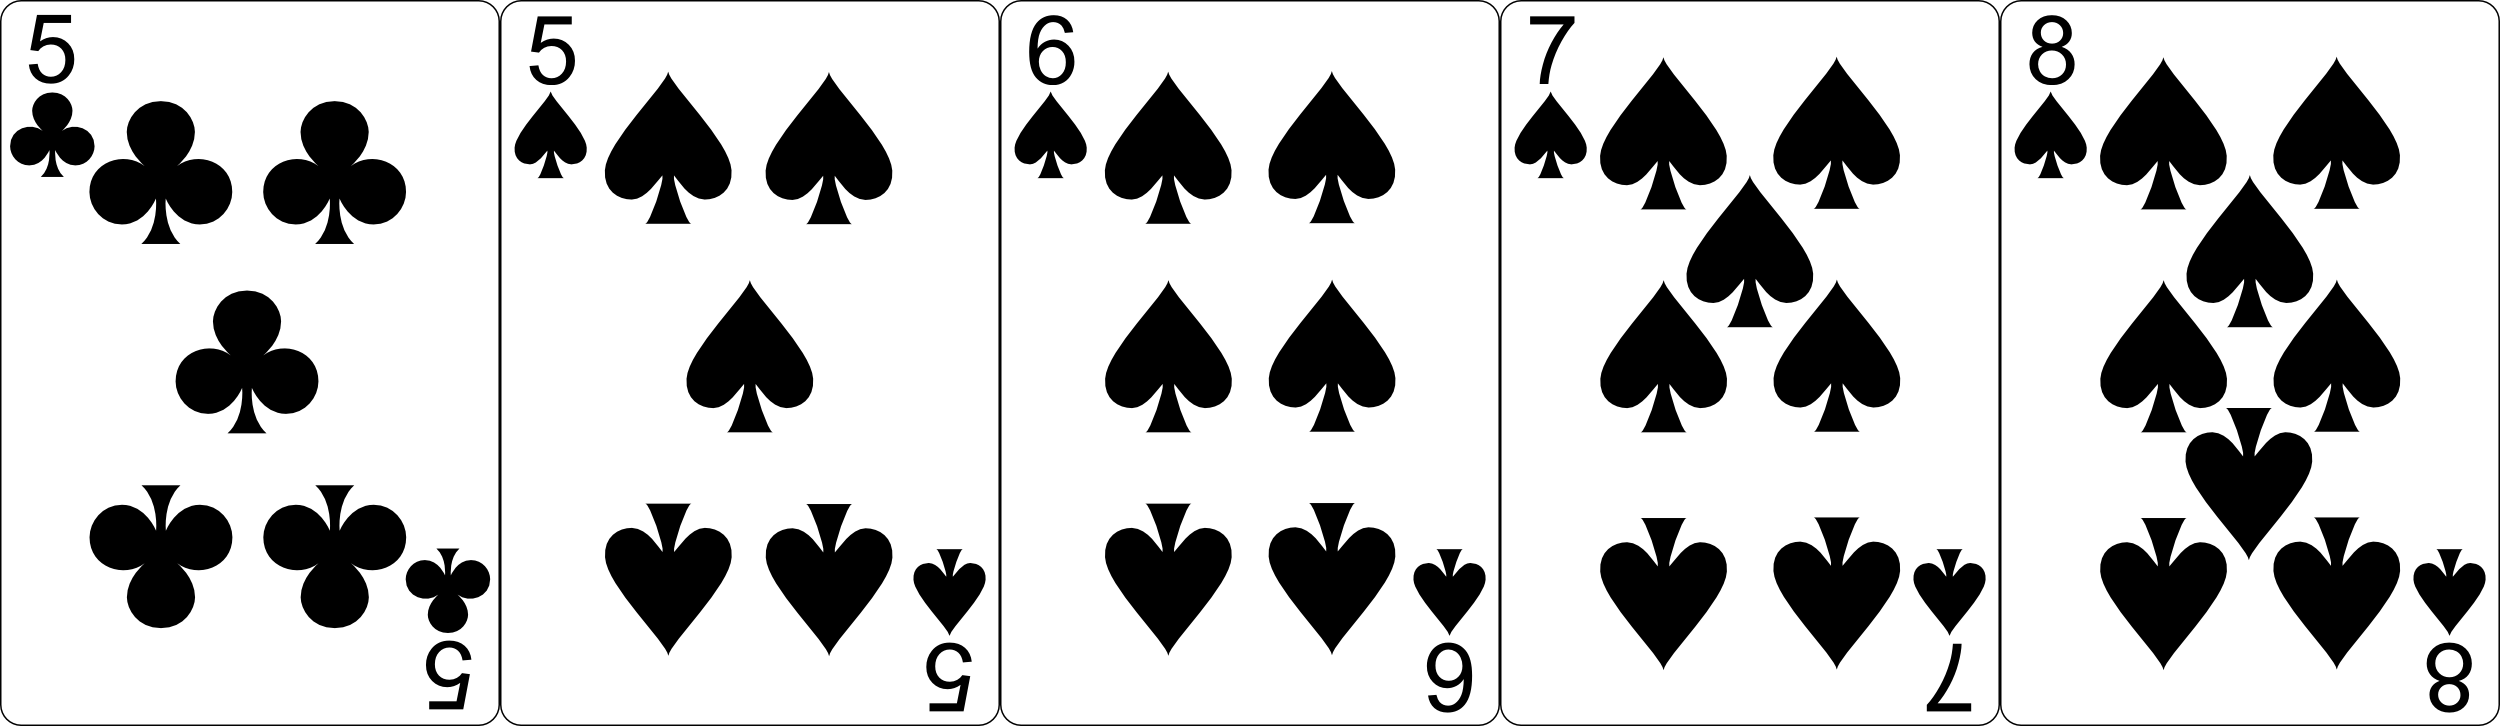
\includegraphics[width=\textwidth]{../img/w05-hands/pair.png}
 \end{minipage}
 \begin{minipage}[c]{\CardCaptionWidth}
  \caption{Par: två kort har samma valör.}
   \label{lab:shuffle:first-picture}
 \end{minipage}
\end{figure}

\begin{figure}[H]
 \begin{minipage}[c]{\CardWidth}
  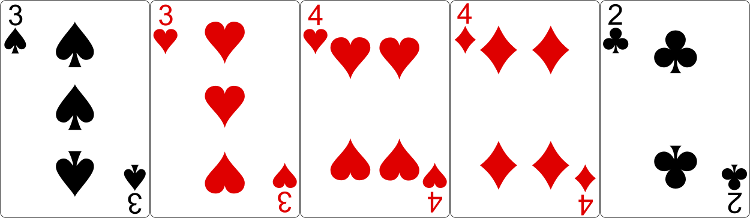
\includegraphics[width=\textwidth]{../img/w05-hands/twopair.png}
 \end{minipage}
 \begin{minipage}[c]{\CardCaptionWidth}
  \caption{Två par: handen har två \emph{olika} par.}
 \end{minipage}
\end{figure}

\begin{figure}[H]
 \begin{minipage}[c]{\CardWidth}
  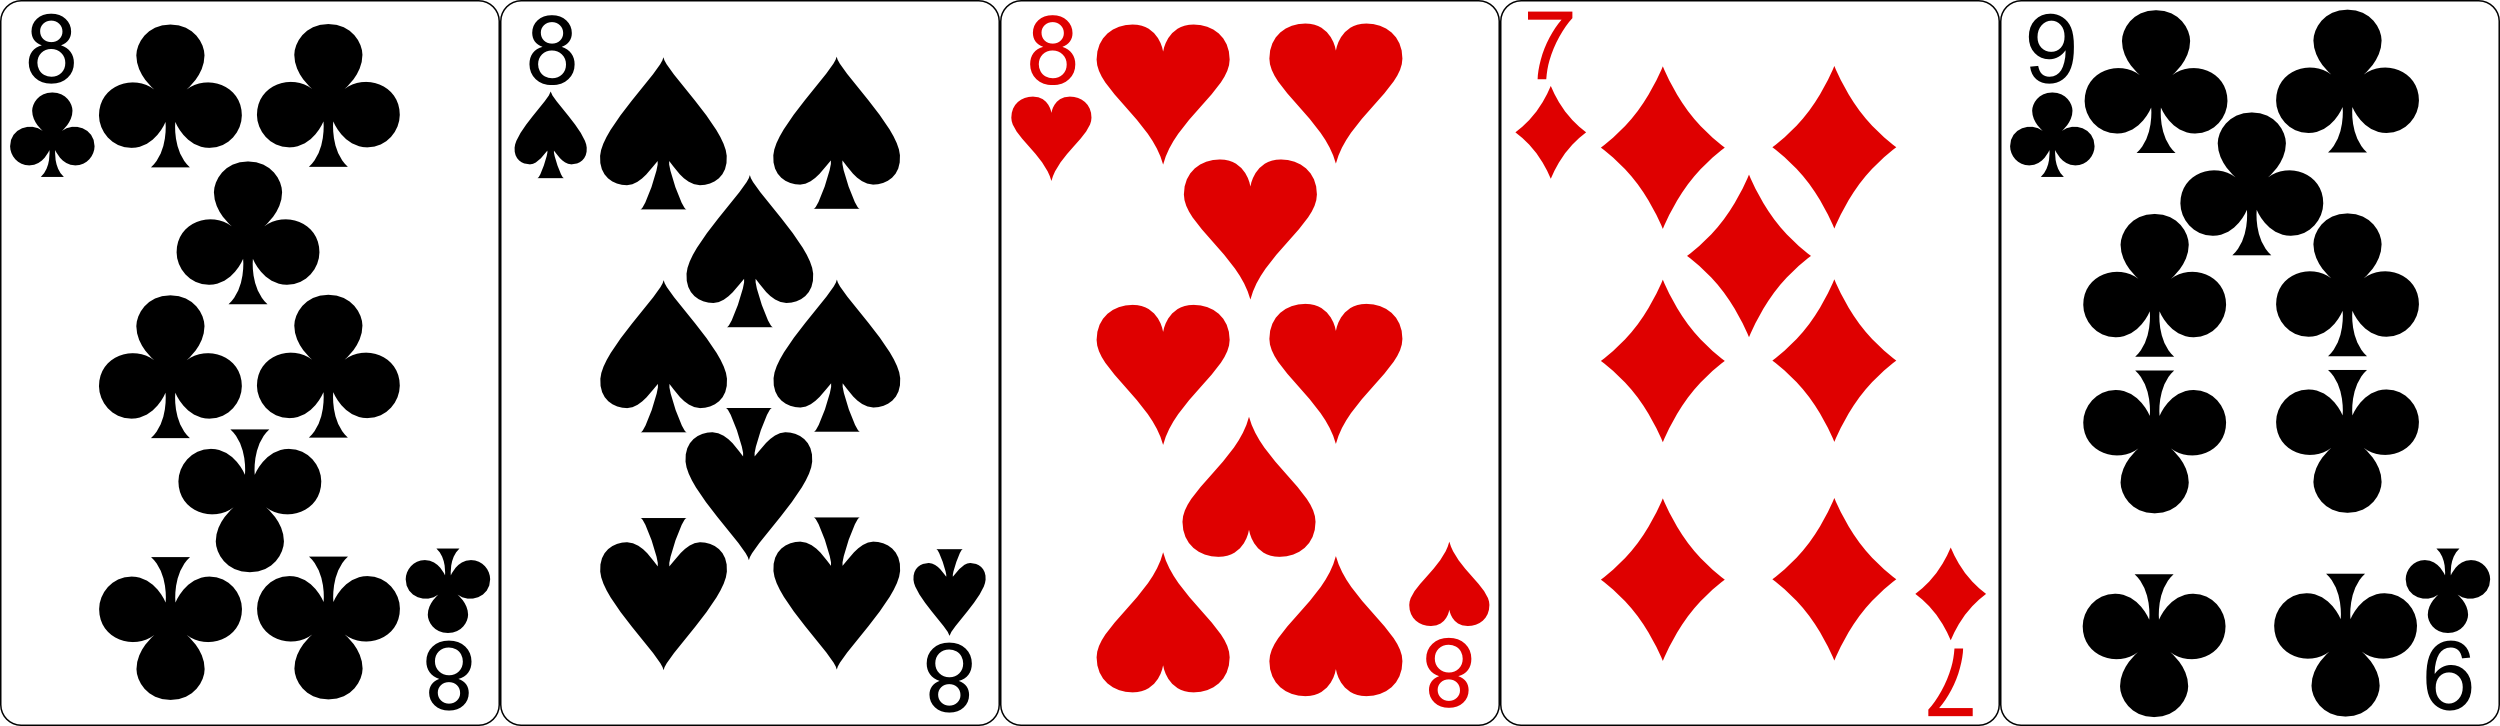
\includegraphics[width=\textwidth]{../img/w05-hands/trips.png}
 \end{minipage}
 \begin{minipage}[c]{\CardCaptionWidth}
  \caption{Triss: tre kort har samma valör.}
 \end{minipage}
\end{figure}

\begin{figure}[H]
 \begin{minipage}[c]{\CardWidth}
  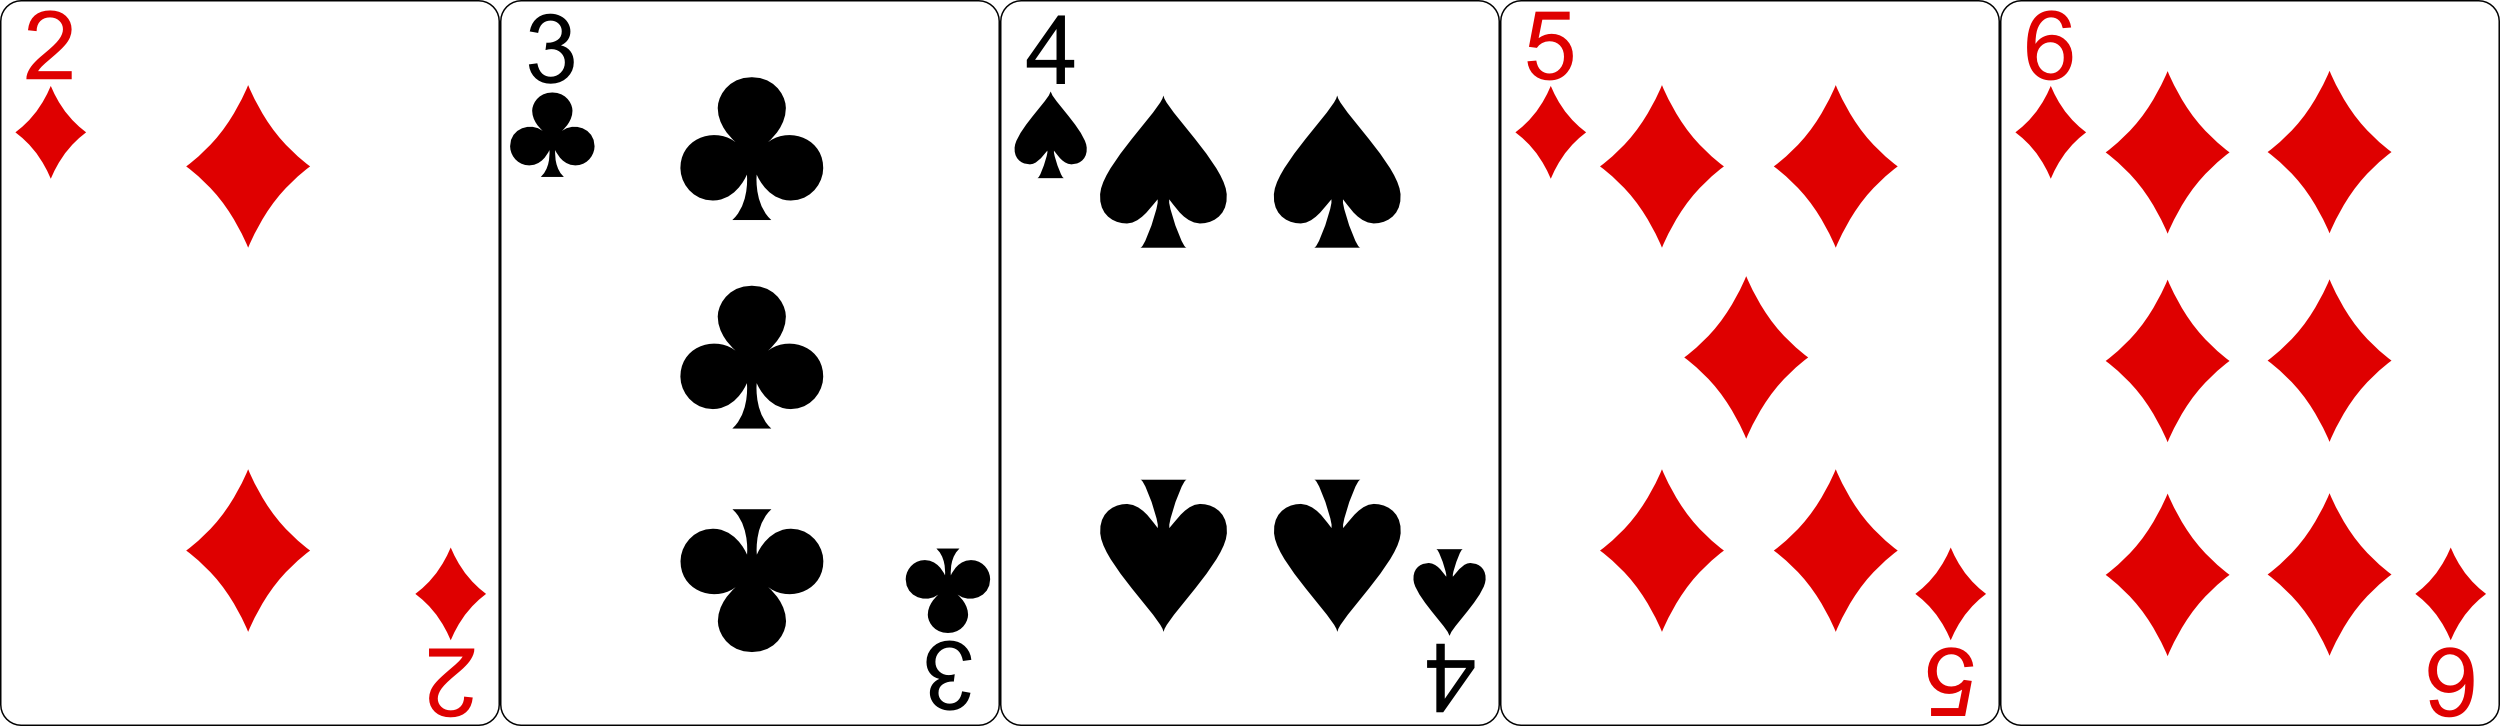
\includegraphics[width=\textwidth]{../img/w05-hands/straight.png}
 \end{minipage}
 \begin{minipage}[c]{\CardCaptionWidth}
  \caption{Stege: kortens valörer bildar en följd, ess kan vara antingen 1 eller 14.}
 \end{minipage}
\end{figure}

\begin{figure}[H]
 \begin{minipage}[c]{\CardWidth}
  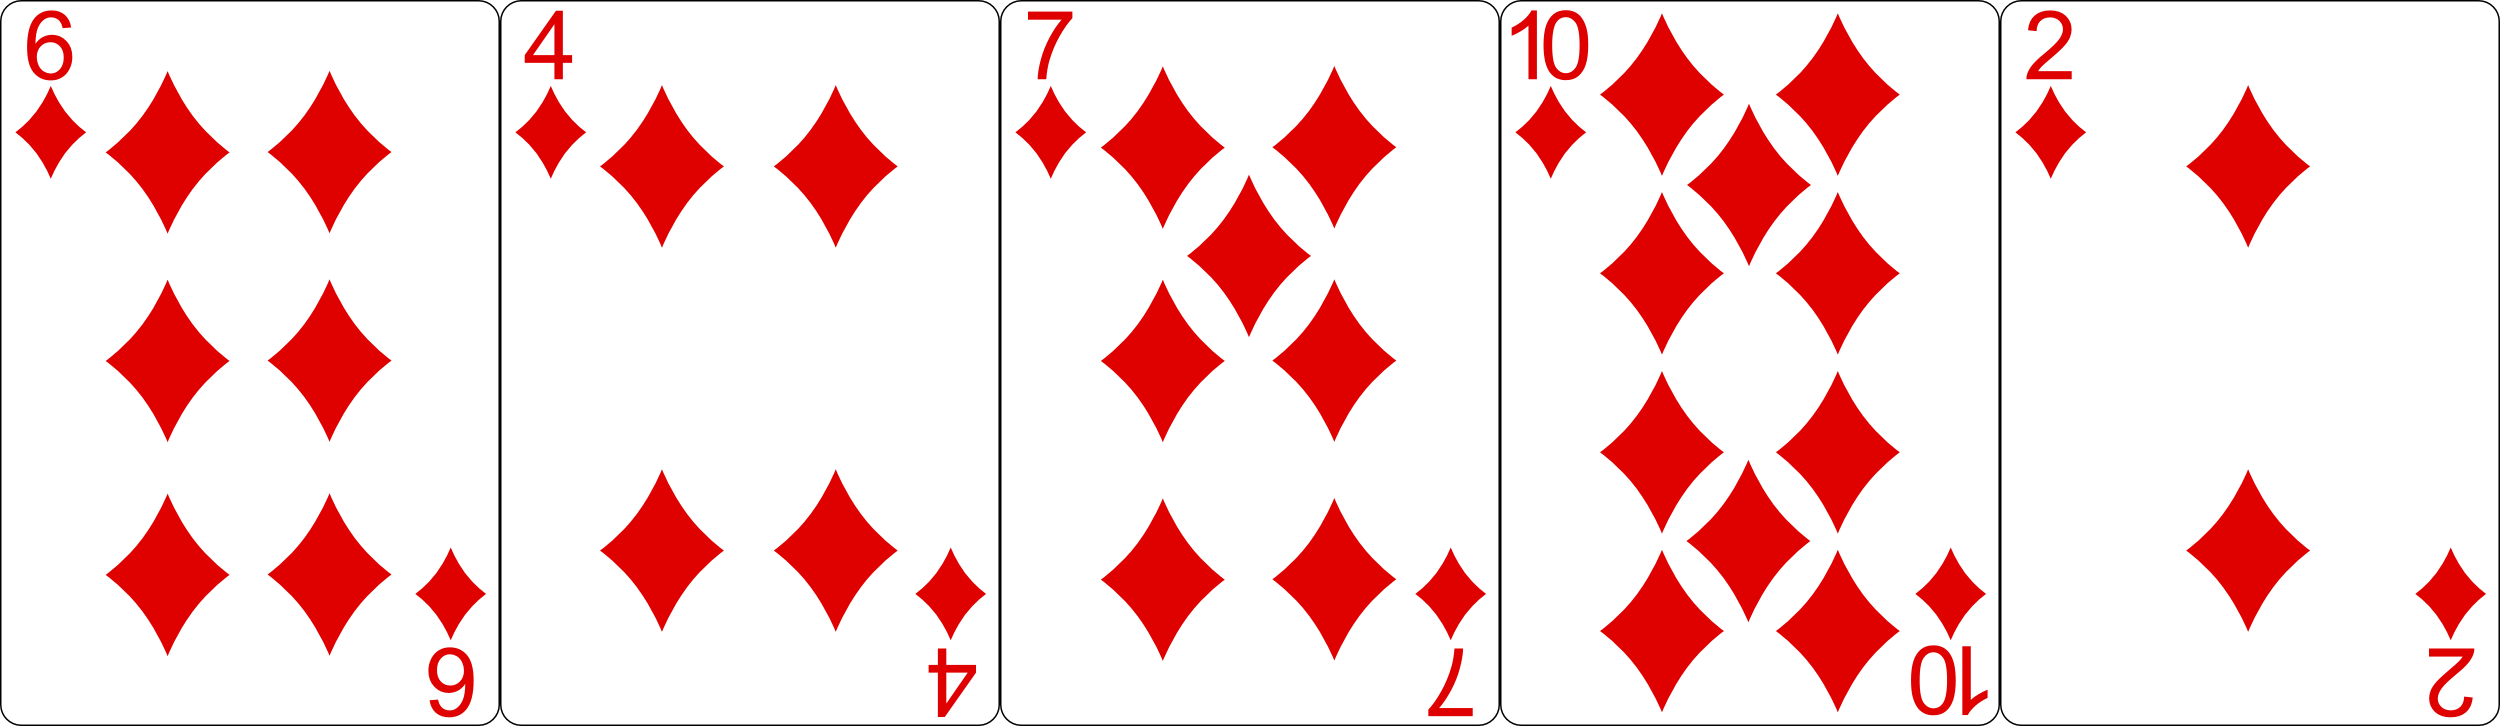
\includegraphics[width=\textwidth]{../img/w05-hands/flush.png}
 \end{minipage}
 \begin{minipage}[c]{\CardCaptionWidth}
  \caption{Färg: alla kort har samma färg.}
 \end{minipage}
\end{figure}

\begin{figure}[H]
 \begin{minipage}[c]{\CardWidth}
  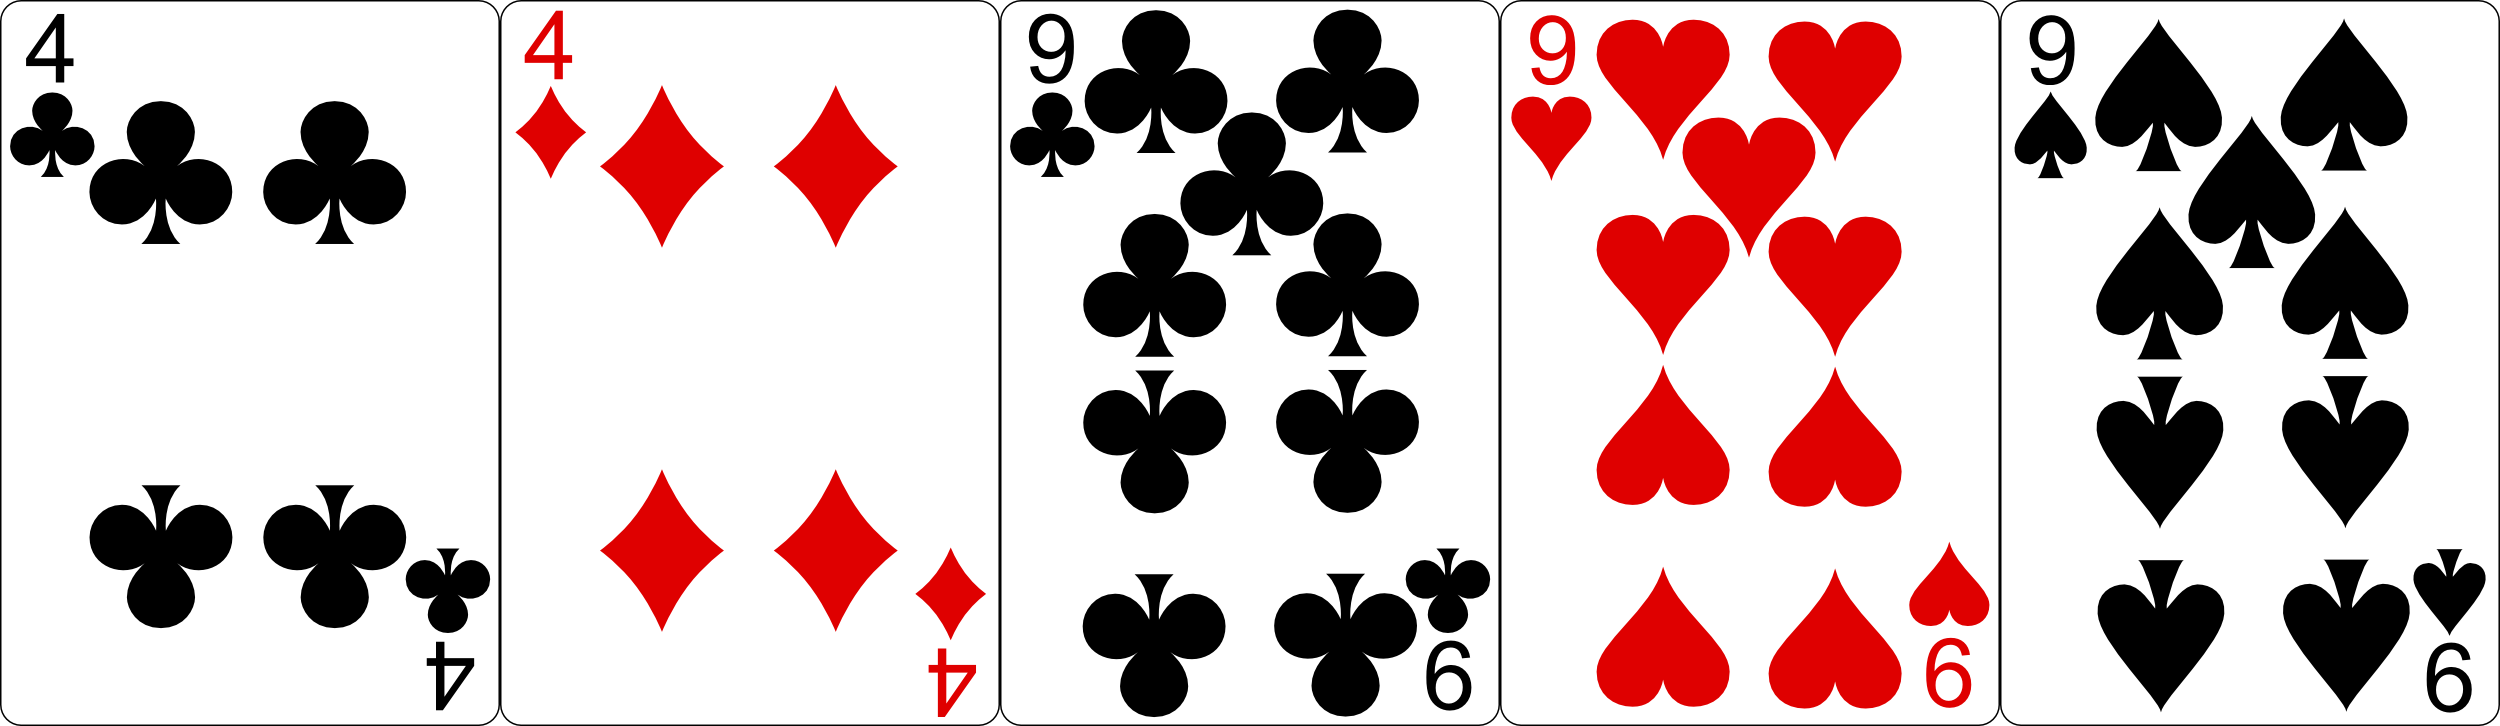
\includegraphics[width=\textwidth]{../img/w05-hands/fullhouse.png}
 \end{minipage}
 \begin{minipage}[c]{\CardCaptionWidth}
  \caption{Kåk: både triss och par.}
 \end{minipage}
\end{figure}

\begin{figure}[H]
 \begin{minipage}[c]{\CardWidth}
  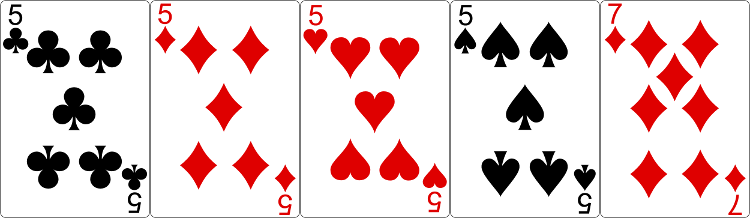
\includegraphics[width=\textwidth]{../img/w05-hands/fours.png}
 \end{minipage}
 \begin{minipage}[c]{\CardCaptionWidth}
  \caption{Fyrtal: fyra kort har samma valör.}
 \end{minipage}
\end{figure}

\begin{figure}[H]
 \begin{minipage}[c]{\CardWidth}
  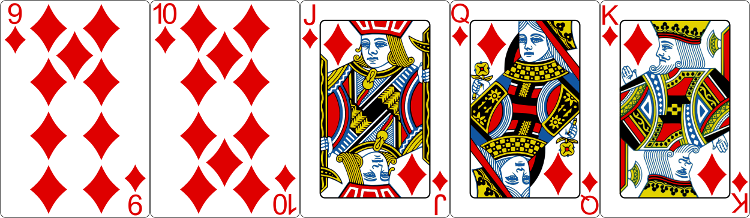
\includegraphics[width=\textwidth]{../img/w05-hands/straightflush.png}
 \end{minipage}
 \begin{minipage}[c]{\CardCaptionWidth}
  \caption{Färgstege: både stege och färg.}
 \end{minipage}
\end{figure}

\begin{figure}[H]
 \begin{minipage}[c]{\CardWidth}
  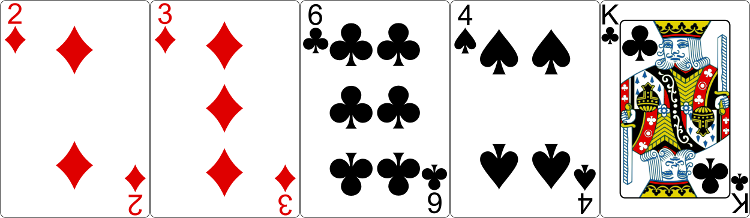
\includegraphics[width=\textwidth]{../img/w05-hands/none.png}
 \end{minipage}
 \begin{minipage}[c]{\CardCaptionWidth}
  \caption{Högt kort: inget mönster finns.}
 \label{lab:shuffle:last-picture}
  \end{minipage}
\end{figure}
